% This is a general template file for the LaTeX package SVJour3
% for Springer journals. Original by Springer Heidelberg, 2010/09/16
%
% Use it as the basis for your article. Delete % signs as needed.
%
% This template includes a few options for different layouts and
% content for various journals. Please consult a previous issue of
% your journal as needed.
%
\RequirePackage{fix-cm}

%
%\documentclass{svjour3}                     % onecolumn (standard format)
%\documentclass[smallcondensed]{svjour3}     % onecolumn (ditto)
\documentclass[smallextended]{svjour3}       % onecolumn (second format)
%\documentclass[twocolumn]{svjour3}          % twocolumn
%
\smartqed  % flush right qed marks, e.g. at end of proof
%
\usepackage{graphicx}
\usepackage{mathtools}
%
% insert here the call for the packages your document requires
%\usepackage{mathptmx}      % use Times fonts if available on your TeX system
%\usepackage{latexsym}
% etc.
%
% please place your own definitions here and don't use \def but
% \newcommand{}{}
%
% Insert the name of "your journal" with
% \journalname{myjournal}
%
\begin{document}

\title{Reliability Budget of CESM using DART
%\thanks{}
}
% Grants or other notes about the article that should go on the front
% page should be placed within the \thanks{} command in the title
% (and the %-sign in front of \thanks{} should be deleted)
%
% General acknowledgments should be placed at the end of the article.

% \subtitle{Do you have a subtitle?\\ If so, write it here}

%\titlerunning{Short form of title}        % if too long for running head

\author{Jonathan Eliashiv        \and
        Aneesh Subramanian \and
        Arthur J. Miller%etc.
}

%\authorrunning{Short form of author list} % if too long for running head

\institute{J. Eliashiv \at
              9500 Gilman Dr. San Diego, CA 92093-0234 \\
            %   Tel.: +123-45-678910\\
            %   Fax: +123-45-678910\\
              \email{jeliashi@ucsd.edu}           %  \\
%             \emph{Present address:} of F. Author  %  if needed
}

\date{Received: date / Accepted: date}
% The correct dates will be entered by the editor

\maketitle

\begin{abstract}
Insert your abstract here. Include keywords, PACS and mathematical
subject classification numbers as needed.
\keywords{First keyword \and Second keyword \and More}
% \PACS{PACS code1 \and PACS code2 \and more}
% \subclass{MSC code1 \and MSC code2 \and more}
\end{abstract}

\section{Introduction}
\label{intro}
The Community Earth Systems Model, CESM, has greatly improved and adapted since its inception, and has come a long way. DART exists. CESM was run with DART for the period of 1970-1981 using ocean temperature and salinity, as well as air temperature and wind data.
Data Assimilation history and DART.
We can use reliability budgets to try to isolate mechanisms of errors. Can we identify structural sources of error in CESM using the data assimilated into it? Are there mechanisms that increase the accuracy? Is there any systematic biases? Is there a threshold to the number of observations needed to assimilate in order to create more accurate assimilations?

\section{Methods}
The purpose of this study is to identify answers for the questions raised above. In order to answer them we must put the model into a framework that can better identify these answers. To do so we need to put the model into a reliability budget to explore the errors. We use Rodwell et al's reliability budget to set the framework which takes observations $o$ and ensemble means prior to assimatlation $m$ and finds the variance as follows:\\

\begin{align}
Var(x) &= \overline{x^2} - \overline{x}^2\nonumber\\
Cov(x,y) &= \overline{xy} - \overline{x}\overline{y}\nonumber\\
Var(m - o) &= Var(m) + Var(o) - 2Cov(m, o)\nonumber\\
\overline{(m-o)^2} &= \overline{m-o}^2 + Var(m) + Var(o) -2Cov(m,o)\label{initDeriv}
\end{align}
We assume that there is minimal if any covariance between model and observation. We also assume that the variance of the model is of order with the ensemble variance, $\overline{e_m^2}$, and assume that model variance is on the order of observation uncertainty, $\overline{e_o^2}$. Per Rodwell's labeling convertion, equation \ref{initDeriv} becomes:
\begin{align}
\overbrace{\overline{(m-o)^2}}^\text{Departure} &= \overbrace{\overline{m-o}^2}^\text{Bias} +\overbrace{\overline{e_m^2}}^\text{Ensemble Variance}+ \overbrace{\overline{e_o^2}}^\text{Observation Uncertainty} \nonumber\\
&\hspace{5mm} + \underbrace{(Var(o) - \overline{e_o^2}) + (Var(m) - \overline{e_m^2}) - 2Cov(m,o)}_\text{Residual}\label{relBudj}
\end{align}
Figure XXXX shows the observation density of all the different variable types assimilated. Each variable uses multiple products from ACARS and XXXX for atmosphere and ocean measurements respectively. The spatial representation of the budget for all the different variables, shown in Figure XXX, shows the residual to be on par in magnitude with the other terms, with opposite sign. 
\subsection{Estimating observation and model error}
It is worthwhile to further breakdown the budget to estimate model and observation ensemble to isolate the overestimation of ensemble variance and observation uncertainty. To do so we assume the bias to have a structure $f(x)$. We define the truth of a variable as $t$.
\begin{align}
    m &\equiv t - e_m +f(x)\nonumber\\
    o &\equiv t - e_o\nonumber\\
    Var(m) &= Var(t) + Var(e_m) + Var(f(x) - 2Cov(t, e_m)\nonumber\\
    &\hspace{5mm}+ 2Cov(t, f(x)) -2Cov(e_m, f(x))\nonumber\\
    &= Var(t) + Var(e_m) + Var(f(x)) + 2Cov(t, f(x))\\
    Var(o) &= Var(t) + Var(e_o) - 2Cov(t, e_o)\nonumber\\
    &= Var(t) + Var(e_o)\nonumber\\
    Cov(m, o) &= Cov(t +f(x), t)\nonumber\\
    &= Var(t) + Cov(f(x), t)\nonumber\\
    Var(m-o) &= Var(e_m) + Var(e_o)+ Var(f(x)) \nonumber\\
    Var(e_o) &= Var(m-o) - Var(m) + Cov(m,o)\label{eoDeriv}
\end{align}
If we assume the systematic error to be approximately linear, we can further derive $e_m$.
\begin{align}
    f(x) &\approx Ax + B\nonumber\\
    Cov(f(x), o) &\approx ACov(x,o)\nonumber\\
    A &\approx \frac{2Cov(m,o) + Var(m-o) -Var(o) -Var(m)}{Cov(x,o)}\\
    Var(f(x)) &= A Var(x)\nonumber\\
    Var(e_m) &= adga
\end{align}
The application of the above derivations from equations XXXX and XXXX are used on the assimilated variables, but negative values of the above estimations are shown in using this analysis, as seen in figure XXX. To further find the limitations of this analysis, it is applied to a Lorenz 63 system as seen in Appendix I.
\subsection{Structural Exploration}
This initial budget from equation \ref{relBudj} can be used to identify the presence of structural mechanisms that either limit or increase error propagation through the model. By limiting the budget to look at all observations for individual measurement types in different spatial dimensions, error can be localized, and likely isolated to particular mechanisms. This study further breaks down the different variables in terms of spatial dimensions and interseasonal indices. Interannual and multidecadal scales cannot be viewed as the data only spans a decade, making large scales views unreliable for lack of data.

\section{Budget Exploration}
Figure XXXX shows equation \ref{relBudj} for Air Temperature in the context of longitude, latitude, height, and time. The temporal exploration shows a cyclical structure with year. To identify the seasonal dependence of the budget, the climatology of the budget is made as seen in figure XXXX. This shows a peak in error during XXX months and trough in XXX months, indicating a slight seasonal dependence, however not nearly as large as that seen by latitude.

Since figure XXX showed a low observational density of measurements in the southern hemisphere, the southern hemisphere peak in error should be explored in context with observation density to determine the leading cause of the error. To do so, the observational effect on the budget is derived as
\begin{align}
    n &\equiv n(\mathbf{x}) = n(t, \theta, \phi, z)\nonumber\\
    R(n) &= R(n(t,\theta,\phi, z)\nonumber\\
    \frac{\partial R}{\partial n} &= \frac{\frac{\partial R}{\partial t}}{\frac{dn}{dt}} + \frac{\frac{\partial R}{\partial \theta}}{\frac{dn}{d\theta}} + \frac{\frac{\partial R}{\partial \phi}}{\frac{dn}{d\phi}} +\frac{\frac{\partial R}{\partial z}}{\frac{dn}{dz}}\label{partialT}\\
    \overline{\frac{\partial R}{\partial n}} &\equiv \frac{\int  n R\mathbf{dx}}{\int  n\mathbf{dx}}\nonumber
\end{align}
where $n$ is observation density, $t$ is time, $\theta$ is longitude, $\phi$ is latitude, $z$ is height, and $R$ is the respective reliability budget term. Using the above derivation, figure XXX shows the effect of observation density on each of the reliability budget values. Observation density has the leading influence on the model, dwarfing all other terms by orders of magnitude.  Therefore any structural component of the budget is subject to changes in the observation density. Since time is the only variable without a large change in observation density, the seasonal dependence is a structural component.

\subsection{Interseasonal Exploration}
As seen in a previous study, using data assimilation in CESM significantly improves the performance of MJO events. It would follow that MJO events would correlate to a drift in model values away from observations. Then CESM would be corrected towards the observations every assimilation period. Figure XXXX shows that MJO events actually decrease the error in observation space, counter to a conventional analysis. To further explore this phenomenna, the budget is split to observe MJO in its different phases. The differences between the resultant budget in each of the different phases and the budget with no MJO events is shown in figures XXXX and XXXX. Figure XXXX shows the effect of longitude to try to isolate whether there is an error reducing process isolated to traveling with the MJO events, whereas figure XXXX shows the effect of temperature during MJO events. With these figures combined a correlation between error and convective processes can be explored, however no significant correlation can be seen.

\section{Discussion}
Throughout this study the effects of data assimilation are explored and understood in the context of structural or mechanistic dependence. The study allows the ability to find systematic biases that grow
\section{Conclusion}

\section{Appendix I - Lorenz 63}

\section{Appendix II - Wind and Ocean measurements in analysis}
% \label{sec:1}
% Text with citations \cite{RefB} and \cite{RefJ}.
% \subsection{Subsection title}
% \label{sec:2}
% as required. Don't forget to give each section
% and subsection a unique label (see Sect.~\ref{sec:1}).
% \paragraph{Paragraph headings} Use paragraph headings as needed.


% % For one-column wide figures use
% \begin{figure}
% % Use the relevant command to insert your figure file.
% % For example, with the graphicx package use
%   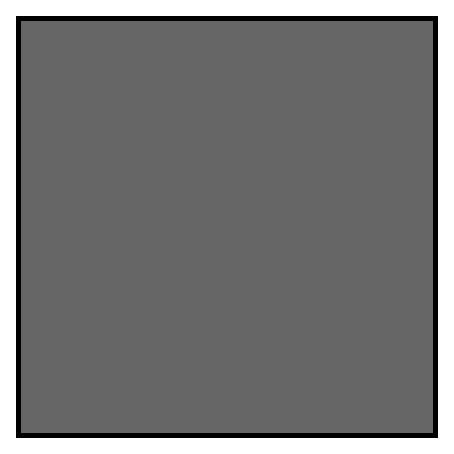
\includegraphics{example.eps}
% % figure caption is below the figure
% \caption{Please write your figure caption here}
% \label{fig:1}       % Give a unique label
% \end{figure}
% %
% % For two-column wide figures use
% \begin{figure*}
% % Use the relevant command to insert your figure file.
% % For example, with the graphicx package use
%   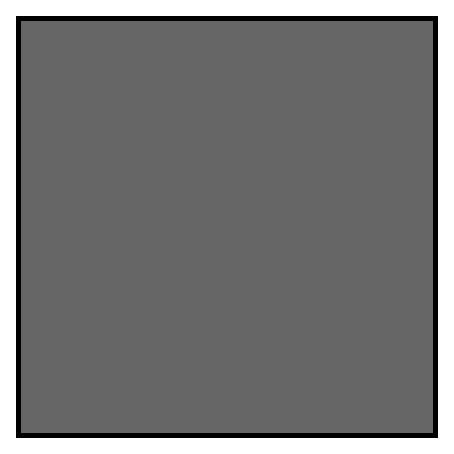
\includegraphics[width=0.75\textwidth]{example.eps}
% % figure caption is below the figure
% \caption{Please write your figure caption here}
% \label{fig:2}       % Give a unique label
% \end{figure*}
% %
% % For tables use
% \begin{table}
% % table caption is above the table
% \caption{Please write your table caption here}
% \label{tab:1}       % Give a unique label
% % For LaTeX tables use
% \begin{tabular}{lll}
% \hline\noalign{\smallskip}
% first & second & third  \\
% \noalign{\smallskip}\hline\noalign{\smallskip}
% number & number & number \\
% number & number & number \\
% \noalign{\smallskip}\hline
% \end{tabular}
% \end{table}


%\begin{acknowledgements}
%If you'd like to thank anyone, place your comments here
%and remove the percent signs.
%\end{acknowledgements}

% BibTeX users please use one of
%\bibliographystyle{spbasic}      % basic style, author-year citations
%\bibliographystyle{spmpsci}      % mathematics and physical sciences
%\bibliographystyle{spphys}       % APS-like style for physics
%\bibliography{}   % name your BibTeX data base

% Non-BibTeX users please use
\begin{thebibliography}{}
%
% and use \bibitem to create references. Consult the Instructions
% for authors for reference list style.
%
\bibitem{RefJ}
% Format for Journal Reference
Author, Article title, Journal, Volume, page numbers (year)
% Format for books
\bibitem{RefB}
Author, Book title, page numbers. Publisher, place (year)
% etc
\end{thebibliography}

\end{document}
% end of file template.tex